\chapter{DISEÑO TECNOLÓGICO}

% ======================================================================
% CAPITULO VI - DISENO TECNOLOGICO
% Alcance: Fases 1 y 2 (OE1 y OE2), que son las implementadas y ejecutadas.
%
% DELIMITACION RESPECTO DEL CAPITULO IV:
% El Capitulo IV justifica la eleccion de cada herramienta y el valor de cada
% umbral con sus matrices de seleccion ponderada y sus citas. Este capitulo NO
% repite esa justificacion: toma los umbrales como especificacion de entrada y
% documenta el dimensionamiento computacional, la seleccion de versiones y
% entornos, la implementacion en codigo y la arquitectura del sistema.
%
% PREAMBULO REQUERIDO EN main.tex (agregar junto a los demas \usepackage):
%   \usepackage{tikz}
%   (las figuras de 6.4 usan solo tikz base: no requieren \usetikzlibrary)
%   \usepackage{listings}
%   \lstset{
%     basicstyle=\ttfamily\scriptsize,
%     columns=fixed, basewidth={0.5em,0.45em}, keepspaces=true,
%     breaklines=true, breakatwhitespace=true, breakindent=0pt,
%     frame=leftline, framerule=0.8pt, framesep=8pt, xleftmargin=12pt,
%     aboveskip=1.2\baselineskip, belowskip=1.0\baselineskip,
%     abovecaptionskip=6pt, showstringspaces=false,
%     captionpos=b, tabsize=2, numbers=none}
%   \renewcommand{\lstlistingname}{Código}
% ======================================================================

Este capítulo documenta la construcción del flujo bioinformático con el que se
ejecutaron las Fases 1 y 2. El Capítulo IV estableció qué
herramientas se emplean, por qué se eligieron frente a sus alternativas y qué
valor toma cada umbral. Este capítulo parte de esas decisiones y no las repite.
Frente a ello, el objetivo de este capítulo es determinar el tamaño de los recursos que el flujo
necesita, seleccionar las versiones y los entornos que lo hacen ejecutable sobre
la infraestructura disponible, implementarlo en código y describir la
arquitectura que resulta de integrar todas sus piezas.

\section{Cálculo de los parámetros y dimensionamiento de los componentes}

El dimensionamiento del flujo bioinformático no consiste en calcular el
volumen de un equipo, sino en determinar cuántos recursos de cómputo,
almacenamiento y tiempo consume cada etapa, y comprobar que esos consumos caben
en la infraestructura disponible. Esta sección establece primero las bases de
diseño, que son el volumen de datos de entrada y los parámetros operativos
heredados del marco metodológico, y a partir de ellas dimensiona cada etapa.

\subsection{Bases de diseño: el conjunto de datos de entrada}

El sistema opera sobre genomas ya ensamblados y agrupados. No procesa lecturas crudas. Esta condición fija las características de la entrada y, con ella, el orden de magnitud de todo el
dimensionamiento posterior. La Tabla~\ref{tab:bases_diseno} resume las
características del conjunto.

\begin{table}[H]
\centering
\small
\caption[Bases de diseño del conjunto de entrada]{Características del conjunto
de bins de entrada, medidas sobre los archivos FASTA de origen.}
\label{tab:bases_diseno}
\begin{tabular}{lr}
\toprule
\textbf{Característica} & \textbf{Valor} \\
\midrule
Bins de entrada                       & 97 \\
Librerías de origen                   & 22 \\
Volumen total de secuencia            & 1.12 Gpb \\
Contigs totales                       & 151\,180 \\
Tamaño mediano por bin                & 4.28 Mpb \\
Tamaño mínimo por bin                 & 0.22 Mpb \\
Tamaño máximo por bin                 & 101.9 Mpb \\
Contigs en el bin más fragmentado     & 41\,610 \\
\bottomrule
\end{tabular}
\end{table}

Dos cifras de esta tabla condicionan el diseño. La primera es el tamaño máximo
de 101.9 Mpb, que corresponde a \texttt{bin-11-71}. Un bin de ese tamaño no es
un genoma bacteriano sino una mezcla, y su presencia en la entrada obliga a que
la primera etapa del flujo sea capaz de procesar archivos un orden de magnitud
mayores que el caso típico. La segunda es el volumen total de 1.12 Gpb, que es
modesto para los estándares de la metagenómica. El cuello de botella del sistema
no está, por tanto, en el tamaño de los datos propios, sino en el tamaño de las
bases de datos de referencia que el flujo debe consultar.

\subsection{Parámetros operativos del diseño}

Los parámetros que gobiernan cada etapa se establecieron en el Capítulo IV junto
con su fundamento. La Tabla~\ref{tab:parametros_operativos} los reúne en la
forma en que quedan codificados en el sistema, que es como variables de
configuración al inicio de cada script de ejecución. El propósito de esta tabla no es
justificarlos de nuevo, sino dejar constancia de la correspondencia exacta entre
el valor definido en la metodología y el valor implementado.

\begin{table}[H]
\centering
\small
\caption[Parámetros operativos implementados]{Parámetros operativos del diseño y
variable con que se implementan. La justificación de cada valor se encuentra en
el Capítulo IV.}
\label{tab:parametros_operativos}
\makebox[\textwidth][c]{%
\begin{tabular}{lllr}
\toprule
\textbf{Fase} & \textbf{Parámetro} & \textbf{Variable en el código} & \textbf{Valor} \\
\midrule
1 & Longitud mínima de contig      & \texttt{MIN\_CONTIG\_LEN}   & 3000 \\
1 & Completitud mínima             & \texttt{MIN\_COMPLETENESS}  & 70 \\
1 & Contaminación máxima           & \texttt{MAX\_CONTAMINATION} & 5 \\
2 & Umbral primario de dRep (MASH) & \texttt{DREP\_PA}           & 0.90 \\
2 & Umbral secundario de dRep (ANI)& \texttt{DREP\_SA}           & 0.95 \\
2 & ANI de confirmación de especie & \texttt{ANI\_ESPECIE}       & 95 \\
2 & Fracción alineada mínima       & \texttt{AF\_ESPECIE}        & 65 \\
\bottomrule
\end{tabular}%
}
\end{table}

Los parámetros se declaran como variables al principio del script y no
aparecen escritos dentro de las llamadas a las herramientas. Esta decisión de
implementación tiene una consecuencia práctica: cambiar un umbral exige editar
una sola línea, y el valor efectivo queda registrado de forma automática en el
archivo de versiones que el propio script ejecutado escribe. El análisis de
sensibilidad del Capítulo VII se apoya en esa propiedad.

\subsection{Dimensionamiento del cómputo}

La cuenta de usuario en el clúster Khipu admite como máximo 32 núcleos, 98 GB de
memoria y 24 horas de ejecución por trabajo. Ese límite es la restricción dura
del dimensionamiento. La Tabla~\ref{tab:dimensionamiento} indica, para cada
etapa, cuál es el recurso crítico y qué decisión de diseño se tomó para que el
consumo quepa dentro de la cuota.

\begin{table}[H]
\centering
\footnotesize
\setlength{\tabcolsep}{4pt}
\caption[Dimensionamiento de cómputo por etapa]{Recurso crítico de cada etapa y
decisión de dimensionamiento adoptada.}
\label{tab:dimensionamiento}
\makebox[\textwidth][c]{%
\begin{tabular}{p{2.4cm}p{2.2cm}p{7.6cm}}
\toprule
\textbf{Etapa} & \textbf{Recurso crítico} & \textbf{Decisión de dimensionamiento} \\
\midrule
Tiara &
Procesador &
Se ejecuta un bin por vez en un bucle, con los 32 núcleos asignados a cada
llamada. El procesamiento secuencial evita que el bin de 101.9 Mpb coincida en
memoria con otros bins grandes \\
\addlinespace
CheckM2 &
Memoria y disco &
Se ejecuta una sola llamada sobre el conjunto completo de bins procariotas, lo
que carga la base de DIAMOND una vez en lugar de una por genoma \\
\addlinespace
GTDB-Tk &
Memoria &
La etapa de colocación filogenética es la de mayor consumo de todo el flujo. Se
fija \texttt{-{}-pplacer\_cpus 1}, con lo que el consumo de esa etapa se acota a
unos 55 GB para el conjunto de marcadores bac120. Con más hilos el consumo crece
por encima de la cuota \\
\addlinespace
GTDB-Tk &
Tiempo y disco &
Se fija \texttt{-{}-skip\_ani\_screen}, que omite el prefiltrado por MASH y
elimina la necesidad de una base de datos adicional. La confirmación de especie
se obtiene igualmente del cálculo interno de ANI \\
\addlinespace
dRep &
Tiempo &
Se reutiliza la evaluación de calidad ya producida por CheckM2 en la Fase 1
mediante \texttt{-{}-genomeInfo}, de modo que dRep no vuelve a estimar
completitud ni contaminación \\
\bottomrule
\end{tabular}%
}
\end{table}

La asignación final de recursos se declara en la cabecera de cada script de ejecución.
Ambas fases solicitan 32 núcleos y 90 GB de memoria, es decir, ocho gigabytes por
debajo del límite máximo de la cuenta. Ese margen es deliberado: el planificador rechaza
el trabajo si la solicitud excede la cuota, y algunas herramientas reservan
memoria adicional fuera del proceso principal. La Fase 1 solicita 24 horas y la
Fase 2, doce.

La etapa de GTDB-Tk merece un comentario aparte porque es la que determina el
dimensionamiento de todo el sistema. La colocación filogenética de los genomas
sobre el árbol de referencia es un procedimiento cuyo consumo de memoria crece
con el número de hilos, no con el número de genomas de consulta. Por ese motivo
la única variable de ajuste disponible es el número de hilos de esa subetapa, y
por ese motivo se fija en uno aunque el resto del flujo disponga de 32. Esta
restricción es también la que impidió construir el árbol \textit{de novo} con el
conjunto completo de referencias del dominio bacteriano, como se documenta en
el Capítulo VII.

\subsection{Dimensionamiento del almacenamiento}

El volumen de datos propios es pequeño frente al de las bases de referencia. La
Tabla~\ref{tab:almacenamiento} lo detalla.

\begin{table}[H]
\centering
\small
\caption[Dimensionamiento del almacenamiento]{Requerimiento de almacenamiento
por componente.}
\label{tab:almacenamiento}
\begin{tabular}{llr}
\toprule
\textbf{Componente} & \textbf{Tipo} & \textbf{Tamaño} \\
\midrule
Bins de entrada                       & Datos propios     & 1.12 Gpb \\
Base de datos de CheckM2 (DIAMOND)    & Insumo de referencia & $\sim$3 GB \\
Base de datos de GTDB R220            & Insumo de referencia & $\sim$110 GB \\
Resultados completos de la Fase 2     & Salida            & 406 MB \\
Alineamiento concatenado bac120       & Salida intermedia & 230 MB \\
\bottomrule
\end{tabular}
\end{table}

La base de GTDB determina por sí sola el requerimiento de disco del proyecto.
Su descompresión desde el archivo comprimido es una operación de larga duración
que debe ejecutarse en el nodo de login, único con acceso a internet, y que
excede la tolerancia de una sesión interactiva. Por ese motivo el script de
preparación de la Fase 2 verifica el espacio disponible antes de iniciar la
descompresión y está diseñado para ejecutarse en un segundo plano.

\section{Selección de materiales, componentes y equipos de la solución}

En un diseño de esta naturaleza los materiales son de tres clases: las versiones
concretas del software, las bases de datos que actúan como insumo de referencia
y el entorno de ejecución que hace reproducible el conjunto. La elección de cada
herramienta ya se justificó en el Capítulo IV. Lo que se selecciona aquí es la
versión, el insumo y el entorno, decisiones que no son metodológicas sino de
implementación, y que en este proyecto resultaron determinantes para que el
flujo funcionara.

\subsection{Versiones de software y compatibilidad}

La Tabla~\ref{tab:versiones} indica la versión empleada de cada herramienta y el
criterio con que se fijó.

\begin{table}[H]
\centering
\footnotesize
\setlength{\tabcolsep}{4pt}
\caption[Versiones de software seleccionadas]{Versiones de software empleadas y
criterio de selección de cada una.}
\label{tab:versiones}
\makebox[\textwidth][c]{%
\begin{tabular}{p{2.2cm}p{1.8cm}p{8.2cm}}
\toprule
\textbf{Componente} & \textbf{Versión} & \textbf{Criterio de selección de la versión} \\
\midrule
GTDB-Tk & 2.6.1 &
Fijada de forma explícita por compatibilidad con el release R220 de la base de
datos. La tabla de compatibilidad oficial de la herramienta vincula cada versión
del programa con un release de datos determinado, y una combinación incorrecta
produce clasificaciones erróneas sin emitir error \\
\addlinespace
Python & 3.11 &
Fijada de forma explícita en todos los entornos. Sin esta restricción el
resolvedor instala Python 3.14, con el que GTDB-Tk no arranca porque la versión
de su biblioteca de validación de datos no es compatible con esa versión \\
\addlinespace
Tiara, CheckM2 & última estable &
Sin restricción de versión. Ninguna de las dos depende de un release externo de
datos versionado \\
\addlinespace
dRep, fastANI, MASH & última estable, Python 3.11 &
Instaladas en un entorno propio con la misma versión de Python, para evitar la misma
clase de incompatibilidad \\
\bottomrule
\end{tabular}%
}
\end{table}

La fijación de la versión de Python es la decisión de selección más importante
del capítulo, por la siguiente razón: el error que produce su ausencia
no se manifiesta durante la instalación sino en la primera ejecución, cuando ya
se han descargado 110 GB de base de datos y se ha encolado un trabajo. Fijarla
convierte un fallo tardío en una condición verificable en el momento de crear el
entorno.

\subsection{Bases de datos como insumo de referencia}

Las bases de datos cumplen en este diseño la función que los insumos cumplen en
un proceso físico: son material externo que el sistema consume y del que depende
la validez del resultado. La Tabla~\ref{tab:insumos} las especifica.

\begin{table}[H]
\centering
\small
\caption[Insumos de referencia del sistema]{Bases de datos empleadas como insumo
de referencia.}
\label{tab:insumos}
\makebox[\textwidth][c]{%
\begin{tabular}{lll}
\toprule
\textbf{Insumo} & \textbf{Versión} & \textbf{Etapa que lo consume} \\
\midrule
Base de datos de CheckM2 & la que distribuye la herramienta & Calidad genómica \\
Base de datos de GTDB            & R220                              & Clasificación taxonómica y ANI \\
\bottomrule
\end{tabular}%
}
\end{table}

La versión del insumo forma parte del resultado. Un genoma clasificado contra
R220 puede recibir un nombre distinto contra un release posterior, porque la
taxonomía del GTDB se reorganiza entre versiones. Por ese motivo el release se
registra en el archivo de versiones de cada ejecución y se declara junto a los
resultados.

\subsection{Entorno de ejecución}

El sistema se ejecuta sobre entornos conda independientes, uno por herramienta.
La separación responde a un conflicto real de dependencias: Tiara, CheckM2 y
GTDB-Tk requieren versiones incompatibles de las mismas bibliotecas, y un
entorno único no resuelve.

La selección de canales de paquetes también fue objeto de una decisión. El canal
\texttt{defaults} de la distribución no compila desde el clúster, lo que
produce un fallo de red durante la creación del entorno. El diseño emplea
únicamente los canales \texttt{conda-forge} y \texttt{bioconda}, y los declara
de forma explícita en cada llamada de creación. El Código~\ref{lst:entorno}
muestra la forma en que se implementa esta decisión junto con la fijación de
versiones.

\begin{lstlisting}[language=bash, caption={Creación del entorno de GTDB-Tk con
versión de herramienta y de Python fijadas, y canales declarados de forma
explícita (extracto de \texttt{02\_setup\_fase2\_khipu.sh}).},
label={lst:entorno}]
# Versiones fijadas: GTDB-Tk al release de los datos y Python a
# una serie compatible. --override-channels evita 'defaults'.
$SOLVER create -y -n gtdbtk --override-channels \
    -c conda-forge -c bioconda \
    "gtdbtk=$GTDBTK_VERSION" "python=$PYTHON_VERSION"
\end{lstlisting}

Para dejar constancia del entorno efectivamente utilizado, el guion de
preparación exporta al final un archivo de bloqueo por cada entorno creado, con
la lista completa de paquetes y sus versiones exactas. Esos archivos se
versionan junto con el código.

\subsection{Plataforma de cómputo}

El sistema se ejecuta en el clúster Khipu de la UTEC, bajo el planificador SLURM.
Se emplea la partición \texttt{standard}, que agrupa los nodos de propósito
general con 32 núcleos y 224 GB de memoria. No se emplean las particiones de
GPU, porque ninguna de las herramientas del flujo aprovecha aceleración gráfica,
ni la partición de memoria ampliada, a la que la cuenta no tiene acceso.

La arquitectura del clúster impone una separación que el diseño debe respetar:
solo el nodo de login tiene acceso a internet, y los nodos de cómputo trabajan
sin conexión. Esto obliga a repartir el sistema en dos clases de programas. Los
guiones de preparación descargan bases de datos y crean entornos, y se ejecutan
de forma interactiva en el login. Los scripts de ejecución ejecutan el análisis y se
envían a la cola, sin requerir conexión alguna.

\section{Integración e implementación de los componentes en la solución final}

Las etapas descritas no funcionan de forma aislada. Esta sección documenta cómo
se encadenan, qué resultado produce cada una, qué resultado de la etapa anterior consume la siguiente
y qué mecanismos garantizan que el encadenamiento no se rompa.

\subsection{Organización del sistema en programas}

El sistema se implementa en seis programas, que se agrupan en tres clases según
dónde y cuándo se ejecutan. La Tabla~\ref{tab:programas} los describe.

\begin{table}[H]
\centering
\footnotesize
\setlength{\tabcolsep}{4pt}
\caption[Programas que componen el sistema]{Programas del sistema, clase a la
que pertenecen y función que cumplen.}
\label{tab:programas}
\makebox[\textwidth][c]{%
\begin{tabular}{p{4cm}p{2.2cm}p{6.6cm}}
\toprule
\textbf{Programa} & \textbf{Clase} & \textbf{Función} \\
\midrule
\texttt{00\_setup\_khipu.sh} & Preparación (login) &
Crea los entornos de Tiara y CheckM2 y descarga la base de datos de CheckM2 \\
\addlinespace
\texttt{01\_prep\_bins.sh} & Preparación (local) &
Normaliza el conjunto de bins de entrada y genera la tabla de trazabilidad \\
\addlinespace
\texttt{02\_setup\_fase2\_khipu.sh} & Preparación (login) &
Crea los entornos de GTDB-Tk y dRep con versiones fijadas y descomprime la base
de GTDB R220 \\
\addlinespace
\texttt{run\_fase1.slurm} & script de ejecución (cola) &
Ejecuta el filtrado por dominio, la evaluación de calidad y la selección \\
\addlinespace
\texttt{run\_fase2.slurm} & script de ejecución (cola) &
Ejecuta la clasificación taxonómica, la desreplicación y el cálculo de prevalencia \\
\addlinespace
\texttt{summarize\_phase1.py}, \texttt{summarize\_phase2.py} & Procesamiento &
Convierten las salidas de cada herramienta en las tablas de decisión del flujo
y en los reportes legibles \\
\bottomrule
\end{tabular}%
}
\end{table}

La separación entre script de ejecución y procesamiento es deliberada. El script de ejecución se
ocupa de activar entornos, invocar herramientas y
verificar condiciones. Los programas de procesamiento contienen la lógica de
decisión del flujo, escrita en Python y empleando únicamente la biblioteca
estándar. Esta última restricción permite ejecutarlos con el intérprete de
cualquiera de los entornos, sin instalar dependencias adicionales.

\subsection{Normalización de la entrada y trazabilidad}

La trazabilidad entre cada genoma y su muestra de origen es un requisito del
diseño, porque la prevalencia espacial de la Fase 2 se calcula sobre esos resultados. El programa de preparación la establece antes de que empiece el
análisis.

Los archivos de origen llevan nombres de la forma \texttt{bin-<N>-<muestra>},
que ya codifican la muestra. El programa los copia a una carpeta limpia,
descarta los ensamblajes por muestra que no son bins y construye una tabla de
correspondencia con la muestra, el número de bin, el número de contigs y la
longitud de cada genoma. El Código~\ref{lst:trazabilidad} muestra el núcleo de
esa operación.

\begin{lstlisting}[language=bash, caption={Extracción de la muestra de origen a
partir del nombre de archivo y registro en la tabla de trazabilidad (extracto de
\texttt{01\_prep\_bins.sh}).}, label={lst:trazabilidad}]
# Parseo del nombre: bin-<N>-<muestra>.fasta
core="${bn%.fasta}"        # bin-1-49
sample="${core##*-}"       # 49
rest="${core%-*}"          # bin-1
binn="${rest##*-}"         # 1
nctg=$(grep -c '^>' "$DEST/$bn" || echo 0)
len=$(grep -v '^>' "$DEST/$bn" | tr -d '\n' | wc -c)
printf "%s\t%s\t%s\t%s\t%s\n" \
       "$bn" "$sample" "$binn" "$nctg" "$len" >> "$MAP"
\end{lstlisting}

El programa verifica al final que el número de genomas procesados sea 97 y emite
una advertencia en caso contrario. Esta comprobación protege contra el error más
probable de esta etapa, que es tomar como origen una carpeta equivocada.

\subsection{Encadenamiento entre etapas}

Las etapas se comunican mediante archivos, no mediante memoria compartida. Cada
etapa escribe un archivo en disco y la siguiente lo lee. La
Tabla~\ref{tab:artefactos} documenta esa cadena, que es la descripción precisa
de cómo la salida de un componente alimenta al siguiente.

\begin{table}[H]
\centering
\footnotesize
\setlength{\tabcolsep}{4pt}
\caption[Archivos que encadenan las etapas]{Archivos de datos que conectan
las etapas del sistema.}
\label{tab:artefactos}
\makebox[\textwidth][c]{%
\begin{tabular}{p{4.3cm}p{2.6cm}p{5.8cm}}
\toprule
\textbf{Archivo} & \textbf{Lo produce} & \textbf{Lo consume} \\
\midrule
\texttt{bin\_rename\_map.tsv} & Preparación &
La Fase 2, para asignar cada genoma a su muestra y calcular prevalencia \\
\addlinespace
\texttt{tiara\_bin\_summary.tsv} & Tiara y su resumen &
La copia selectiva de bins procariotas hacia la entrada de CheckM2 \\
\addlinespace
\texttt{quality\_report.tsv} & CheckM2 &
La selección de la Fase 1 y, más adelante, dRep en la Fase 2 \\
\addlinespace
\texttt{phase1\_selection.tsv} & Resumen de la Fase 1 &
El reporte de la Fase 1. Documenta el motivo de descarte de cada bin \\
\addlinespace
\texttt{phase1\_selected\_genomes/} & Resumen de la Fase 1 &
La Fase 2 completa. Es su única entrada de secuencias \\
\addlinespace
\texttt{genomeInfo.csv} & Resumen de la Fase 2 &
dRep, para evitar que recalcule la calidad de los genomas \\
\addlinespace
\texttt{Cdb.csv}, \texttt{Wdb.csv} & dRep &
El cálculo de linajes, representantes y prevalencia \\
\bottomrule
\end{tabular}%
}
\end{table}

Dos elementos de esta cadena resuelven problemas de integración concretos.

El primero es la carpeta de genomas seleccionados. La Fase 2 no recibe una lista
de nombres ni un filtro que deba volver a aplicar, sino una carpeta que contiene
exactamente los genomas que superaron la Fase 1. De ese modo el criterio de
selección se aplica una sola vez, en el lugar donde está definido, y no puede
divergir entre fases.

El segundo es el archivo de información de genomas. La herramienta de
desreplicación evalúa por omisión la calidad de cada genoma con su propio
procedimiento, lo que duplicaría un cálculo ya realizado y podría además
descartar genomas que la Fase 1 había aceptado. El diseño evita ambos problemas
convirtiendo el reporte de CheckM2 al formato que la herramienta espera y
desactivando sus filtros propios, como muestra el Código~\ref{lst:drep}.

\begin{lstlisting}[language=bash, caption={Reutilización de la evaluación de
calidad de la Fase 1 y desactivación de los filtros propios de dRep (extracto de
\texttt{run\_fase2.slurm}).}, label={lst:drep}]
# genomeInfo.csv a partir de CheckM2 (Fase 1): evita que dRep
# vuelva a estimar completitud y contaminacion.
python "$SCRIPTS_DIR/summarize_phase2.py" genomeinfo \
    --genomes-dir "$DREP_INPUT" --bin-ext "$BIN_EXT" \
    --checkm2 "$CHECKM2_REPORT" \
    --out "$RESULTS/genomeInfo.csv"

# -comp 0 -con 100: desactiva el filtro propio de dRep, ya
# aplicado en la Fase 1 (>70 % compl., <5 % contaminacion).
dRep dereplicate "$DREP_OUT" \
    -g "$DREP_INPUT"/*."$BIN_EXT" \
    -p "$THREADS" \
    -pa "$DREP_PA" -sa "$DREP_SA" \
    --S_algorithm fastANI \
    -comp 0 -con 100 \
    --genomeInfo "$RESULTS/genomeInfo.csv"
\end{lstlisting}

\subsection{Implementación de los script de ejecuciónes}

Cada script de ejecución declara primero los recursos que solicita al planificador del clúster y
después la configuración del análisis. El Código~\ref{lst:sbatch} reproduce la
cabecera de la Fase 1, que materializa el dimensionamiento de la
Sección 6.1.3.

\begin{lstlisting}[language=bash, caption={Cabecera de solicitud de recursos al
planificador (extracto de \texttt{run\_fase1.slurm}).}, label={lst:sbatch}]
# Limites de la cuenta: 32 cores, 98 GB RAM, 24 h por trabajo.
#SBATCH --job-name=fase1_estela
#SBATCH --partition=standard
#SBATCH --nodes=1
#SBATCH --ntasks=1
#SBATCH --cpus-per-task=32
#SBATCH --mem=90G
#SBATCH --time=24:00:00
#SBATCH --output=fase1_%j.out
#SBATCH --error=fase1_%j.err
\end{lstlisting}

La implementación incorpora tres mecanismos de robustez que conviene documentar
porque responden a condiciones propias de esta plataforma.

El primero es el modo de terminación ante error. Los scripts se ejecutan
con interrupción ante el primer fallo y con propagación del error a través del \textit{pipeline}, pero sin la opción que aborta ante variables no definidas. Esa opción,
que sería deseable, resulta incompatible con el sistema de módulos del clúster,
que referencia una variable de entorno sin definirla previamente. El
Código~\ref{lst:robustez} muestra la solución adoptada y el comentario que la
documenta en el propio archivo.

\begin{lstlisting}[language=bash, caption={Configuración de terminación ante
error, compatible con el sistema de módulos del clúster (extracto de
\texttt{run\_fase1.slurm}).}, label={lst:robustez}]
# NO usar 'set -u' (nounset): Lmod referencia LD_PRELOAD sin
# definir y aborta la carga de modulos en Khipu.
set -eo pipefail
export LD_PRELOAD="${LD_PRELOAD:-}"
\end{lstlisting}

El segundo es un bloque de comprobaciones previas que se ejecuta antes de
cualquier cálculo. Verifica que exista la carpeta de bins, que contenga
archivos, que la base de datos esté descargada y que el entorno conda haya
quedado disponible tras cargar el módulo. Cada comprobación fallida termina el
trabajo con un mensaje que indica qué hacer. La finalidad es que un error de
configuración se manifieste en los primeros segundos y no después de horas de
cola y cómputo.

El tercero es el registro automático de versiones. Antes de empezar, cada
script de ejecución escribe un archivo con la fecha, el identificador del trabajo, el
nodo asignado, los umbrales efectivos y la versión de cada herramienta
consultada al propio programa. Ese archivo acompaña a los resultados y es la
evidencia de reproducibilidad que se reporta en el Capítulo VII.

\subsection{Control de versiones}

El código, las tablas de resultados y los archivos de bloqueo de los entornos se
mantienen en un repositorio de control de versiones. Los archivos de gran tamaño
que no aportan a la reproducibilidad, como el alineamiento concatenado de 230 MB,
quedan excluidos de forma explícita y se conservan solo en el almacenamiento
local. Esta separación mantiene el repositorio manejable sin perder la capacidad
de reconstruir el análisis.

\section{Representación gráfica de la solución y su verificación}

Esta sección traduce las decisiones de las secciones anteriores a dos
representaciones. La primera describe el flujo de datos, es decir, qué
transformación sufre la información en cada etapa. La segunda describe la
arquitectura de cómputo, es decir, dónde se ejecuta cada pieza y por qué.

\subsection{Diagrama de flujo del sistema}

La Figura~\ref{fig:pfd} representa el sistema como una secuencia de operaciones
unitarias conectadas por corrientes de datos. Cada bloque corresponde a una etapa
de transformación, cada flecha representa un archivo de los declarados en la
Tabla~\ref{tab:artefactos} y las cifras indican el número de genomas que atraviesa
cada punto del flujo.

\begin{figure}[H]
\centering
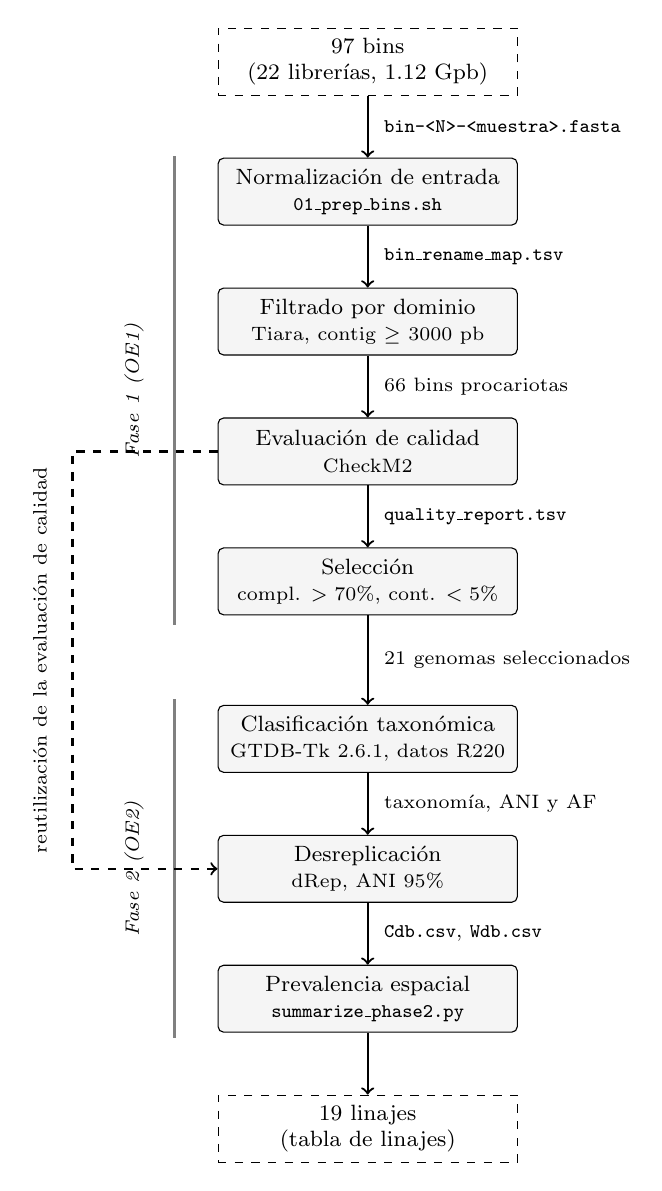
\begin{tikzpicture}[
  font=\footnotesize,
  proc/.style={
    rectangle,
    draw,
    rounded corners=2pt,
    minimum width=3.8cm,
    minimum height=0.85cm,
    align=center,
    fill=gray!8
  },
  data/.style={
    rectangle,
    draw,
    dashed,
    minimum width=3.8cm,
    minimum height=0.85cm,
    align=center
  },
  arr/.style={
    ->,
    thick
  },
  lbl/.style={
    font=\scriptsize,
    midway,
    right=4pt,
    fill=white,
    inner sep=1.5pt
  },
  fase/.style={
    very thick,
    gray
  },
  reutil/.style={
    ->,
    dashed,
    thick
  }
]

% =========================================================
% ETAPAS
% =========================================================

\node[data] (in) at (0,0)
  {97 bins\\(22 librerías, 1.12 Gpb)};

\node[proc] (prep) at (0,-1.65)
  {Normalización de entrada\\
   \scriptsize\texttt{01\_prep\_bins.sh}};

\node[proc] (tiara) at (0,-3.30)
  {Filtrado por dominio\\
   \scriptsize Tiara, contig $\geq$ 3000 pb};

\node[proc] (ckm) at (0,-4.95)
  {Evaluación de calidad\\
   \scriptsize CheckM2};

\node[proc] (sel) at (0,-6.60)
  {Selección\\
   \scriptsize compl. $>70\%$, cont. $<5\%$};

% --- Separación entre fases ---

\node[proc] (gtdb) at (0,-8.60)
  {Clasificación taxonómica\\
   \scriptsize GTDB-Tk 2.6.1, datos R220};

\node[proc] (drep) at (0,-10.25)
  {Desreplicación\\
   \scriptsize dRep, ANI $95\%$};

\node[proc] (prev) at (0,-11.90)
  {Prevalencia espacial\\
   \scriptsize\texttt{summarize\_phase2.py}};

\node[data] (out) at (0,-13.55)
  {19 linajes\\(tabla de linajes)};


% =========================================================
% CORRIENTE PRINCIPAL
% =========================================================

\draw[arr]
  (in) -- node[lbl] {\texttt{bin-<N>-<muestra>.fasta}} (prep);

\draw[arr]
  (prep) -- node[lbl] {\texttt{bin\_rename\_map.tsv}} (tiara);

\draw[arr]
  (tiara) -- node[lbl] {66 bins procariotas} (ckm);

\draw[arr]
  (ckm) -- node[lbl] {\texttt{quality\_report.tsv}} (sel);

\draw[arr]
  (sel) -- node[lbl] {21 genomas seleccionados} (gtdb);

\draw[arr]
  (gtdb) -- node[lbl] {taxonomía, ANI y AF} (drep);

\draw[arr]
  (drep) -- node[lbl] {\texttt{Cdb.csv}, \texttt{Wdb.csv}} (prev);

\draw[arr]
  (prev) -- (out);


% =========================================================
% FASE 1
% =========================================================

\draw[fase]
  (-2.45,-1.20) -- (-2.45,-7.15);

\node[
  font=\scriptsize\itshape,
  rotate=90,
  anchor=south
]
at (-2.72,-4.18)
{Fase 1 (OE1)};


% =========================================================
% FASE 2
% =========================================================

\draw[fase]
  (-2.45,-8.10) -- (-2.45,-12.40);

\node[
  font=\scriptsize\itshape,
  rotate=90,
  anchor=south
]
at (-2.72,-10.25)
{Fase 2 (OE2)};


% =========================================================
% REUTILIZACIÓN DE LA EVALUACIÓN DE CALIDAD
% =========================================================

\draw[reutil]
  (ckm.west)
  -- (-3.75,-4.95)
  -- (-3.75,-10.25)
  -- (drep.west);

\node[
  font=\scriptsize,
  rotate=90,
  anchor=south,
  fill=white,
  inner sep=2pt
]
at (-4.00,-7.60)
{reutilización de la evaluación de calidad};

\end{tikzpicture}

\caption[Diagrama de flujo del sistema]{
Diagrama de flujo del sistema implementado. Los bloques continuos representan
etapas de transformación y los bloques discontinuos, las corrientes de entrada
y salida. Las etiquetas sobre las flechas indican los archivos de datos que
conectan las etapas. La flecha discontinua lateral representa la reutilización
de la evaluación de calidad de la Fase 1 por parte de la desreplicación de la
Fase 2, descrita en la Sección 6.3.3.
}
\label{fig:pfd}
\end{figure}

El diagrama muestra que el flujo es secuencial, con una única conexión entre
fases: la reutilización de la evaluación de calidad. Esta conexión evita repetir
el cálculo de calidad antes de la desreplicación.

\subsection{Arquitectura de cómputo}

La Figura~\ref{fig:arquitectura} representa dónde se ejecuta cada pieza. La
división entre el nodo de login y los nodos de cómputo no es un detalle de
operación sino una restricción de diseño, porque determina qué programas pueden
descargar insumos y cuáles deben encontrarlos ya disponibles.

\begin{figure}[H]
\centering
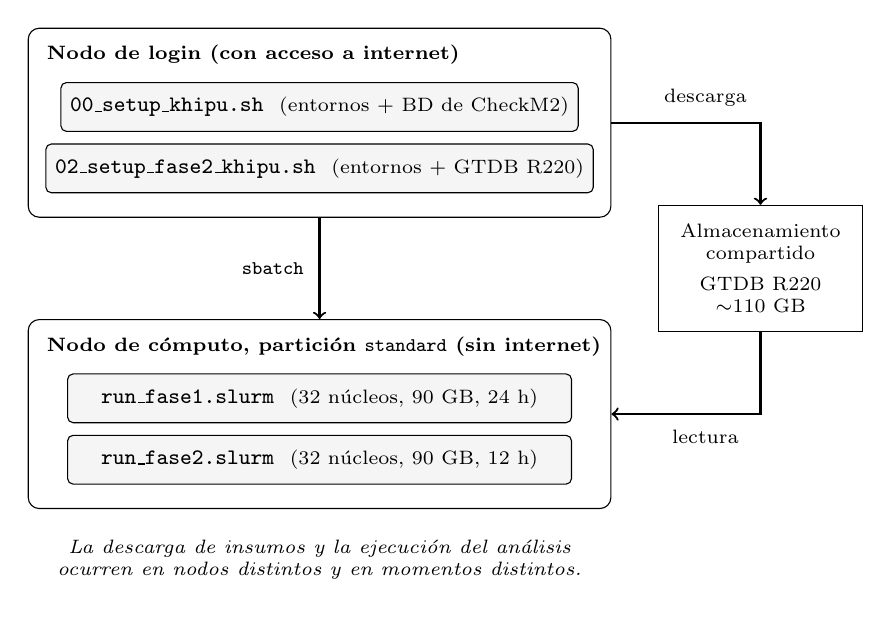
\begin{tikzpicture}[
  font=\footnotesize,
  zona/.style={rectangle, draw, rounded corners=4pt, minimum width=7.4cm,
               minimum height=2.4cm},
  caja/.style={rectangle, draw, rounded corners=2pt, fill=gray!8,
               minimum width=6.4cm, minimum height=0.62cm, align=center},
  disco/.style={rectangle, draw, minimum width=2.6cm, minimum height=1.6cm,
                align=center, font=\scriptsize},
  arr/.style={->, thick}
]

% --- Nodo de login ---
\node[zona] (login) at (0, 1.5) {};
\node[font=\scriptsize\bfseries, anchor=north west]
      at ([shift={(0.12,-0.10)}]login.north west)
      {Nodo de login (con acceso a internet)};
\node[caja] at (0, 1.70)
      {\texttt{00\_setup\_khipu.sh}\ \ \scriptsize(entornos + BD de CheckM2)};
\node[caja] at (0, 0.92)
      {\texttt{02\_setup\_fase2\_khipu.sh}\ \ \scriptsize(entornos + GTDB R220)};

% --- Nodo de computo ---
\node[zona] (compute) at (0, -2.2) {};
\node[font=\scriptsize\bfseries, anchor=north west]
      at ([shift={(0.12,-0.10)}]compute.north west)
      {Nodo de cómputo, partición \texttt{standard} (sin internet)};
\node[caja] at (0, -2.00)
      {\texttt{run\_fase1.slurm}\ \ \scriptsize(32 núcleos, 90 GB, 24 h)};
\node[caja] at (0, -2.78)
      {\texttt{run\_fase2.slurm}\ \ \scriptsize(32 núcleos, 90 GB, 12 h)};

% --- Almacenamiento compartido ---
\node[disco] (alm) at (5.6, -0.35)
      {Almacenamiento\\compartido\\[3pt] GTDB R220\\$\sim$110 GB};

% --- Relaciones ---
\draw[arr] (login.south) -- node[font=\scriptsize, midway, left=2pt]
      {\texttt{sbatch}} (compute.north);
\draw[arr] (login.east) -- (5.6, 1.5) -- (alm.north);
\node[font=\scriptsize, anchor=south] at (4.9, 1.58) {descarga};
\draw[arr] (alm.south) -- (5.6, -2.2) -- (compute.east);
\node[font=\scriptsize, anchor=north] at (4.9, -2.28) {lectura};

\node[font=\scriptsize\itshape, align=center] at (0, -4.05)
      {La descarga de insumos y la ejecución del análisis\\
       ocurren en nodos distintos y en momentos distintos.};

\end{tikzpicture}
\caption[Arquitectura de cómputo del sistema]{Arquitectura de cómputo del
sistema sobre el clúster Khipu. Los programas de preparación se ejecutan de
forma interactiva en el nodo de login, único con acceso a internet, y dejan los
entornos y las bases de datos en el almacenamiento compartido. Los scripts de ejecución
se envían a la cola con \texttt{sbatch} y se ejecutan en un nodo de cómputo sin
conexión, que solo lee lo que la etapa de preparación dejó disponible.}
\label{fig:arquitectura}
\end{figure}

\subsection{Verificación de la correspondencia entre el diagrama y la implementación}

Las dos figuras anteriores describen un sistema que existe y que se ejecutó. La
correspondencia entre ambas y el código puede comprobarse de forma directa. Cada
bloque de la Figura~\ref{fig:pfd} corresponde a una invocación identificable
dentro de uno de los dos scripts de ejecución, y cada archivo rotulado sobre las
flechas corresponde a un archivo que el sistema escribe en disco y que se
conserva en el repositorio junto con los resultados. Las cifras de genomas que
atraviesan cada etapa provienen de la ejecución real y coinciden con las que se
reportan en el Capítulo VII.

Los guiones completos, con todas sus comprobaciones y mensajes, se presentan en
el Anexo correspondiente. Los extractos incluidos en este capítulo recogen las
decisiones de diseño relevantes y omiten el código de verificación y de reporte,
que no aporta información ingenieril adicional.
